A torus can not have a hyperbolic structure, it has naturally a flat structure as the quotient $\mathbb{R}^2 / \mathbb{Z}^2$.
This changes when one study the one ponctured torus. It is a torus $S$ where we choose a point $p$ and remove it (or just marked it).

The construction of this object can be done in two manier at least.
For the first construction, one have to choose a hyperbolic octogone where one side have length $0$ and the two other one $l$, then we sew the border of two of this octogone which give a pair of pant. Finally we can glued with a twist $\tau$ to have the one ponctured torus.

A second construction is given by the representation. Given two hyperbolic isomorphism of $\mathbb{H}$ $A$ and $B$ with different fixed point on $\delta \mathbb{H}$ and with $H := ABA^{-1}B^{-1}$ the commutator should be a parabolic element.

A fundamental domaine is given by the following image:


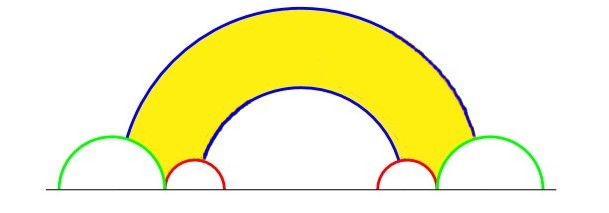
\includegraphics{Image/OnceTorusFundamentalDomaine.jpg}

Given two generators $\alpha$ and $\beta$ of $\pi_1(S)$, two closed curves non homotopically trivial which intersect one, one can parametrize all other lamination.
Indeed a given lamination $\lambda \in \mathcal{ML}$ is determined by the couple $(i(\alpha,\lambda),i(\beta,\lambda))$ where $i(.,.)$ is the geometric intersection number.
